\section{Experiments}
\label{natisand:sect:exp}

\natisand must satisfy two properties to be practical: (i) it must mitigate
real-world vulnerabilities by blocking the associated exploits, and
(ii) it must introduce a limited overhead compared to a scenario where
no protection is applied. In the experimental evaluation, we first
show our solution is able to protect web applications relying on
binary programs and shared libraries affected by high severity
vulnerabilities (Section~\ref{subnatisand:sect:exploit-mitigation}), then we
investigate the performance of our approach
(Section~\ref{subsect:performance-eval}).
Both tests use a server with Ubuntu 22.04 LTS, an AMD Ryzen 3900X CPU,
64 GB RAM, and 2 TB SSD.

\subsection{Exploit mitigation}
\label{subnatisand:sect:exploit-mitigation}

To conduct our analysis we built a representative sample of
vulnerabilities targeting executables and libraries widely used in web
applications. We identified the 32 CVEs reported in
Table~\ref{table-cve}. The entries are separated into three classes:
Arbitrary Code Execution (ACE), Arbitrary File Overwrite (AFO), and
Local File Inclusion (LFI). The list of vulnerable utilities includes
programs used to compress files (e.g., GNU Tar, RAR, Zip), to process
multimedia (e.g., FFmpeg, GraphicsMagick, ImageMagick), database
drivers (e.g., SQLite), and also Machine Learning libraries (e.g.,
Lightning, Sockeye, TensorFlow). We highlight that the vulnerabilities
affect popular open source modules with 2.6M downloads/week available
from the npm and {\tt deno.land/x} archives. Concrete examples are
sharp and fluent-ffmpeg from npm, or flat and sqlite from {\tt
  deno.land/x}.

\begin{table}[!t]
	\setlength{\tabcolsep}{3mm}
	\begin{tabular*}{\columnwidth}{ l l l l l}
	  \toprule
	  {\bf Class} & {\bf CVE Id} & {\bf Utility} & {\bf Type} & {\bf Use case}\\
          \midrule
	  \multirow{25}{*}{ACE}                     & CVE-2016–3714    & ImageMagick    & bin & Image processing    \\
						    & CVE-2019-5063    & OpenCV         & lib & Computer Vision     \\
						    & CVE-2019-5064    & OpenCV         & lib & Computer Vision     \\
						    & CVE-2020-6016    & GNSockets      & lib & P2P networking      \\ 
						    & CVE-2020-6017    & GNSockets      & lib & P2P networking      \\ 
						    & CVE-2020-6018    & GNSockets      & lib & P2P networking      \\
						    & CVE-2020-17541   & libjpeg-turbo  & lib & Compress image      \\
						    & CVE-2020-24020   & FFmpeg         & lib & Video processing    \\
						    & CVE-2020-24995   & FFmpeg         & lib & Video processing    \\
						    & CVE-2020-29599   & ImageMagick    & bin & Image processing    \\
						    & CVE-2021-3246    & libsndfile     & lib & Audio encoding      \\
						    & CVE-2021-3781    & Ghostscript    & bin & PDF processing      \\
							& CVE-2021-4118    & Lightning      & lib & Machine learning    \\
						    & CVE-2021-20227   & SQLite         & lib & Query database      \\
						    & CVE-2021-21300   & Git            & bin & Clone repository    \\
						    & CVE-2021-22204   & ExifTool       & bin & Extract metadata    \\
						    & CVE-2021-37678   & TensorFlow     & lib & Machine learning    \\
							& CVE-2021-43811   & Sockeye        & lib & Translation         \\
						    & CVE-2022-0529    & Unzip          & bin & Decompress archive  \\
						    & CVE-2022-0530    & Unzip          & bin & Decompress archive  \\
							& CVE-2022-0845    & Lightning      & lib & Machine learning    \\
						    & CVE-2022-1292    & OpenSSL        & bin & Verify certificate  \\
						    & CVE-2022-2068    & OpenSSL        & bin & Verify certificate  \\
						    & CVE-2022-2274    & OpenSSL        & lib & Cryptography        \\
						    & CVE-2022-2566    & FFmpeg         & bin & Video processing    \\
	  \midrule
	  \multirow{4}{*}{AFO}  & CVE-2016-6321    & GNU Tar        & bin & Decompress archive  \\
							& CVE-2017-1000472 & POCO           & lib & Common libraries    \\
						    & CVE-2019-20916   & Pip            & bin & Dependency fetch    \\
						    & CVE-2022-30333   & UnRAR          & bin & Decompress archive  \\
	  \midrule
	  \multirow{3}{*}{LFI}  & CVE-2016-1897    & FFmpeg         & bin & Video processing    \\
						    & CVE-2016-1898    & FFmpeg         & bin & Video processing    \\
						    & CVE-2019-12921   & GraphicsMagick & bin & Image processing    \\
	  \bottomrule
	\end{tabular*}
	\caption{\label{table-cve} Sample of CVEs mitigated by \natisand}
\end{table}


First, we checked that public Proofs of Concept of the CVEs in
Table~\ref{table-cve} successfully exploit the vulnerable version of
the utilities. Then, we analyzed whether the vulnerabilities were
exploitable sending the malicious payload through the JS module
interface, and confirmed the feasibility of the attack. The {\em Node
  compatibility mode} was leveraged to execute in Deno the modules
downloaded from npm. We finally repeated the experiment activating the
security functions provided by \natisand, and verified that the attack was
no longer successful, while the application was still able to serve
benign requests (i.e., no functionality loss). The only change we
introduced in the experiment was the specification of a security
policy through the {\tt native-sandbox} CLI argument. The policy was
generated using the tool described in
Section~\ref{sect:sci-ffi-policy-generation}. No modification to the
web application, nor its dependencies, was required to benefit from
the new sandboxing capabilities.


From a security perspective it is worth mentioning that \natisand can
mitigate attacks at multiple levels. For instance, in CVE-2022-2566 a
heap out-of-bound memory bug exists in FFmpeg. The goal of the
attacker is to achieve Arbitrary Code Execution sending to the web
application a malicious {\tt MP4} payload. \natisand denies the compromised
component attempts to access confidential files, open reverse shells,
interact with privileged services through IPC, and transfer data to
unauthorized network hosts. We point out that, while sandboxing limits
the privileges an attacker can gain from exploiting a vulnerable
program, it cannot eliminate vulnerabilities, nor it can
make infeasible to use them in an exploit chain.


\subsection{Performance evaluation}
\label{subsect:performance-eval}

To assess the performance of \natisand we considered a broad set of
programs, including several GNU Core Utilities, executables to process
multimedia, database drivers, and Object Character Recognition
engines. The goal is twofold: (i) evaluate the slowdown compared to a
scenario where no protection is available (i.e., regular Deno), and
(ii) compare \natisand with well known sandboxing and isolation frameworks.
In the following we first investigate the impact on executables, then
we analyze libraries.

\subsubsection{Executables}

In the first batch of experiments we analyze the overhead associated
with executables. Compared to the default scenario where no protection
is available, \natisand spawns each program in a dedicated subprocess with
its own set of constrained ambient rights. A handful of
general purpose sandboxers can be adopted to achieve a comparable
degree of protection by wrapping the execution of each subprocess with the chosen sandboxing utility. In our evaluation, we considered {\em
  Minijail}~\cite{minijail} and {\em Sandbox2}~\cite{sandbox2}.
Minijail is a tool used in ChromeOS and Android to launch and sandbox
other programs based on the set of arguments specified, while Sandbox2
is a C++ library written by Google that can be used to sandbox entire
programs or portions of them. Both Minijail and Sandbox2 support
multiple containment techniques, such as the introduction of dedicated
user ids, restriction of the Linux capabilities, introduction of
policy-based Seccomp filters, and isolation based on Linux namespaces.

\paragraph{Benchmark I}
%
In the first benchmark we implemented a JS application to test the
execution of 17 common Linux utilities with
four configurations: Deno, \natisand, Minijail, and Sandbox2. The
application uses {\tt Deno.run()} to spawn each utility in a
subprocess, and it leverages {\tt Deno.bench()} to determine the duration of each request. The
function ensures that each measure is statistically robust, as it
automatically performs a dynamic number of rounds based on the
duration of the test (i.e., the shorter the test duration, the higher
the number of repetitions). The results are shown in
Table~\ref{table:common-linux-utils} (tests are ordered by increasing
execution time). As expected, the cost of activating the sandbox is
amortized with the increase in the test duration. The tests also show
that \natisand suffers from a smaller performance degradation compared to
Minijail and Sandbox2. This aspect is particularly evident for
short-lived utilities. The reason is that our approach is integrated
by design and, contrary to the other solutions, leverages lightweight
technologies that introduce a smaller performance footprint.

\begin{table}[!t]
	\centering
    \setlength{\tabcolsep}{3mm}
	\begin{tabular*}{0.8\columnwidth}{l r r r r r}
		\toprule
		{\bf Utility} & {\bf Deno \scriptsize{[ms]}} & {\bf Minijail} & {\bf Sandbox2} & {\bf \natisand}\\
		\midrule
		b2sum   & 2.37      & 7.19x     & 9.37x & \bf{2.88x}    \\
		cut     & 2.52      & 7.11x     & 8.97x & \bf{2.86x}    \\
		sum     & 2.61      & 7.00x     & 8.25x & \bf{2.87x}    \\
		tac     & 2.76      & 6.51x     & 8.21x & \bf{2.34x}    \\
		wc      & 2.97      & 6.25x     & 7.69x & \bf{2.44x}    \\
		dd      & 3.60      & 5.29x     & 6.26x & \bf{2.23x}    \\
		seq     & 3.80      & 5.02x     & 5.96x & \bf{2.13x}    \\
		shuf    & 4.29      & 4.68x     & 5.55x & \bf{2.17x}    \\
		ls      & 4.75      & 3.72x     & 4.68x & \bf{1.76x}    \\
		factor  & 5.03      & 4.06x     & 5.03x & \bf{1.86x}    \\
		join    & 5.20      & 4.08x     & 5.18x & \bf{2.05x}    \\
		head    & 6.73      & 3.16x     & 3.85x & \bf{1.56x}    \\
		ping    & 12.20     & 2.27x     & 2.79x & \bf{1.47x}    \\
		sort    & 14.37     & 1.44x     & 1.77x & \bf{1.43x}    \\
		dig     & 22.14     & 1.71x     & 2.15x & \bf{1.17x}    \\
		wget    & 53.24     & 1.18x     & 1.42x & \bf{1.13x}    \\
		curl    & 81.27     & 1.23x     & 1.24x & \bf{1.16x}    \\
		\bottomrule
	\end{tabular*}
	\caption{\label{table:common-linux-utils} Average execution time
	  for common Linux utilities}
\end{table}
%
\begin{figure}[!t]
	\begin{subfigure}{0.48\columnwidth}
		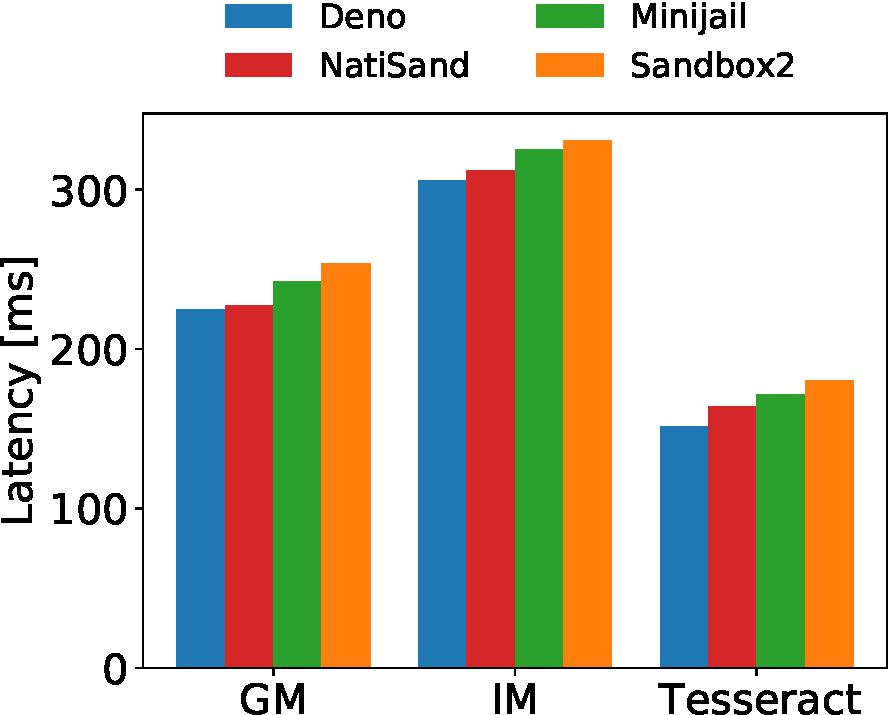
\includegraphics[width=\columnwidth]{chapters/natisand/fig/cropped-summary-subprocess-latency}
	\end{subfigure}%
	\hspace{0.5em}
	\begin{subfigure}{0.48\columnwidth}
		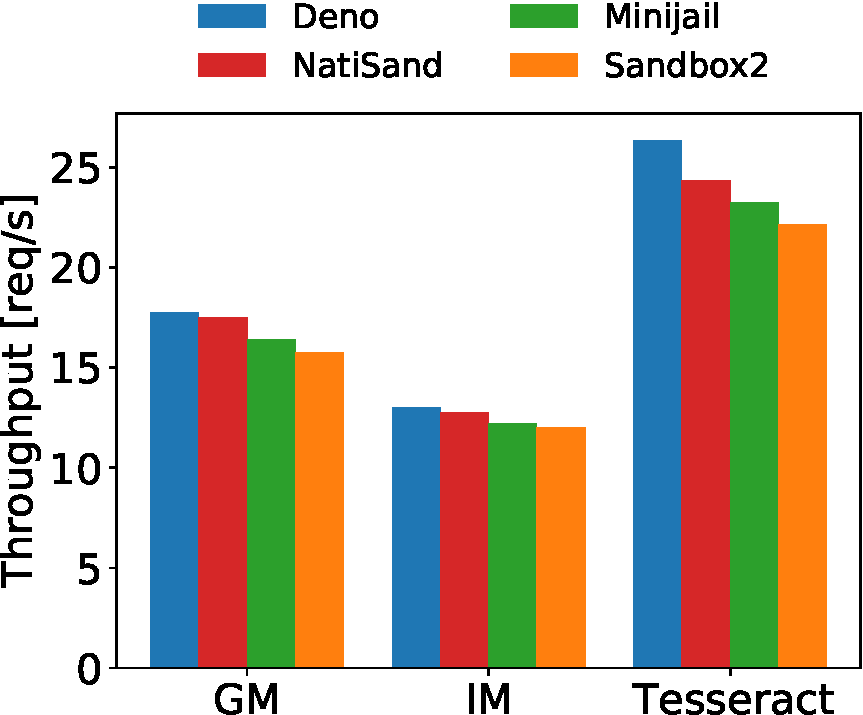
\includegraphics[width=\columnwidth]{chapters/natisand/fig/cropped-summary-subprocess-throughput}
	\end{subfigure}
	\caption[{Average latency and throughput of subprocess-based
	  microservices}]{
	  Average latency and throughput for microservices that execute
	  subprocesses
	}
	\label{fig:subprocess-lat-through}

\end{figure}

\paragraph{Benchmark II}
%
While the experiments part of Benchmark I focus on the server side
scenario, with Benchmark II we wanted to show the overhead experienced
by a remote client. To this end, we used three microservices,
each representing a real use case scenario of high performance native
programs. Two microservices rely on GraphicsMagick and ImageMagick, to
perform a {\em sharpen} operation on images input by the client, while
the third microservice relies on Tesseract to perform Optical
Character Recognition on a second sequence of images input by the
client. Similarly to the previous case, the test was repeated for each
of the four configurations: Deno, \natisand, Minijail, and Sandbox2. This
time the HTTP benchmarking tool {\em wrk} was used to measure the
performance of each microservice.  Network bandwidth and latency are 1
Gbps and 10 ms, respectively, while 100 warmup requests were carried
out. Figure~\ref{fig:subprocess-lat-through} shows the average latency
and the throughput observed over a period of 30 seconds. The results
once again confirm the previous analysis, as longer durations make the
cost to setup the native sandbox less relevant. It is worth to mention
that \natisand exhibits lower overhead compared to Minijail and Sandbox2,
with approximately 5 to 10 ms less latency for each microservice.


\paragraph{Usability}
%
Although general purpose sandboxers can be used to restrict the
permissions associated with executables, to provide a protection
comparable to \natisand: (i) they force the developer to introduce changes in
the web application, and (ii) they require to understand in depth the
techniques used by the kernel to restrict ambient rights (e.g.,
capabilities, namespaces, Seccomp filters). Another problem is that to
restrict IPC and network with Minijail and Sandbox2 it is necessary to
leverage namespaces, which are characterized by coarser granularity
than \natisand policies.



\subsubsection{Libraries}

In the second batch of experiments we analyze the overhead associated
with libraries. Contrary to the default JS runtime behavior, \natisand
transparently executes native library functions in dedicated contexts
with limited ambient rights. A modern, valuable alternative approach
to isolate libraries is to compile them to WebAssembly (Wasm), a
standardized, portable binary instruction format executed in a memory
safe, sandboxed environment. This approach has gained considerable
attention recently, as browsers such as Firefox have used it to
retrofit some of their components to safely interface with native
libraries~\cite{RLBox}.

\paragraph{Benchmark III}
%
Similarly to Benchmark I, we implemented a JS application to highlight
the overhead experienced on the server when native libraries are
executed. In this case three configurations are evaluated: Deno, \natisand,
and Wasm. The application tests the operations provided by four
popular libraries: (i) libxml2, to open and query XML data, (ii) libpng, to read metadata information and verify the
signature of a png image, (iii) opus to encode and create an audio
trace, and (iv) sqlite3, to open and query the Northwind
database. Test durations were again measured with {\tt Deno.bench()},
and the results are reported in
Table~\ref{table:native-lib-overhead}. Deno
exhibits a consistent performance advantage for operations that
require up to 30 microseconds. However, \natisand proves to be more
efficient than Wasm, which in turn is affected by a substantial
overhead in almost every test. This difference is due to the nature of
Wasm; while there have been improvements, the just-in-time
compiled language~\cite{wasm-compilation-pipeline}
remains slower than its native counterpart. Remarkable are the cases
of opus and sqlite3, which used {\tt nativeCall} and demonstrate its
efficiency.

\paragraph{Benchmark IV}
%
To understand the slowdown perceived by a remote client, we exposed
the functions of the libpng, opus, and sqlite3 libraries with
microservices. For each of them, we configured the client to send the
input to the server, and measured the latency and throughput using
{\em wrk} (as explained in Benchmark II setup). The results are
visualized in Figure~\ref{fig:native-lib-latecy-throughput}. Once
again the client observes a small degradation of
latency and throughput when using \natisand instead of Deno, but the
overhead is far less noticeable compared to the results discussed in
Benchmark III. Conversely, Wasm is affected by a significant
degradation of latency. This is due to the just-in-time compilation of Wasm, and the additional memory
management required to exchange data between the JS application and
Wasm.

\begin{table}[!t]
	\centering
	\setlength{\tabcolsep}{3.2mm}
	\begin{tabular*}{0.7\columnwidth}{l r r r r}
		\toprule
		{\bf Test} & {\bf Deno \scriptsize{[$\mu$s]}} & {\bf Wasm} & {\bf \natisand}\\
		\midrule
		libxml2 (open)  & 9.33      & 8.96x     & \bf{2.51x}    \\
		libxml2 (query)	& 11.53     & 4.35x     & \bf{1.63x}    \\
		libpng (verify) & 11.58     & 13.34x    & \bf{9.61x}    \\
		libpng (info)   & 28.33     & 12.63x    & \bf{9.39x}    \\
		opus (encode)   & 58.67     & 2.03x     & \bf{1.55x}    \\
		opus (create)   & 203.72    & 1.70x     & \bf{1.64x}    \\         
		sqlite3 (open)  & 63.62     & 5.68x     & \bf{1.54x}    \\
		sqlite3* (query) & 143.98    & 2.43x     & \bf{1.51x}    \\ 

		\bottomrule
	\end{tabular*}
	\caption[Average execution time for common native libraries]{
		\label{table:native-lib-overhead} Average execution time for
		common native libraries (* marks the use of {\tt nativeCall})
	}
\end{table}
%
\begin{figure}[t!]
	\begin{subfigure}{0.47\columnwidth}
		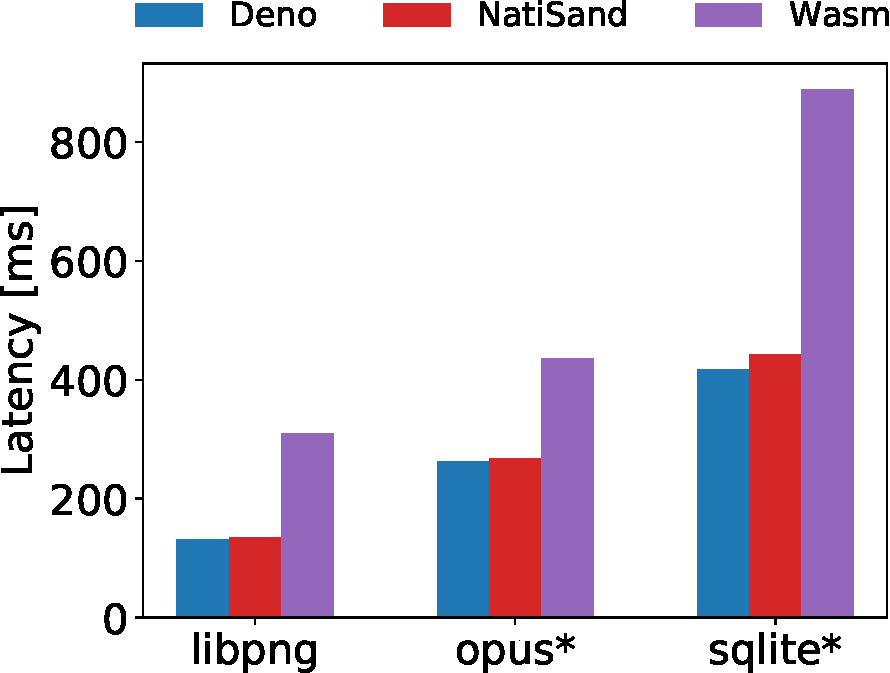
\includegraphics[width=\columnwidth]{chapters/natisand/fig/cropped-summary-ffi-latency.pdf}
	\end{subfigure}%
	\hspace{1em}
	\begin{subfigure}{0.47\columnwidth}
		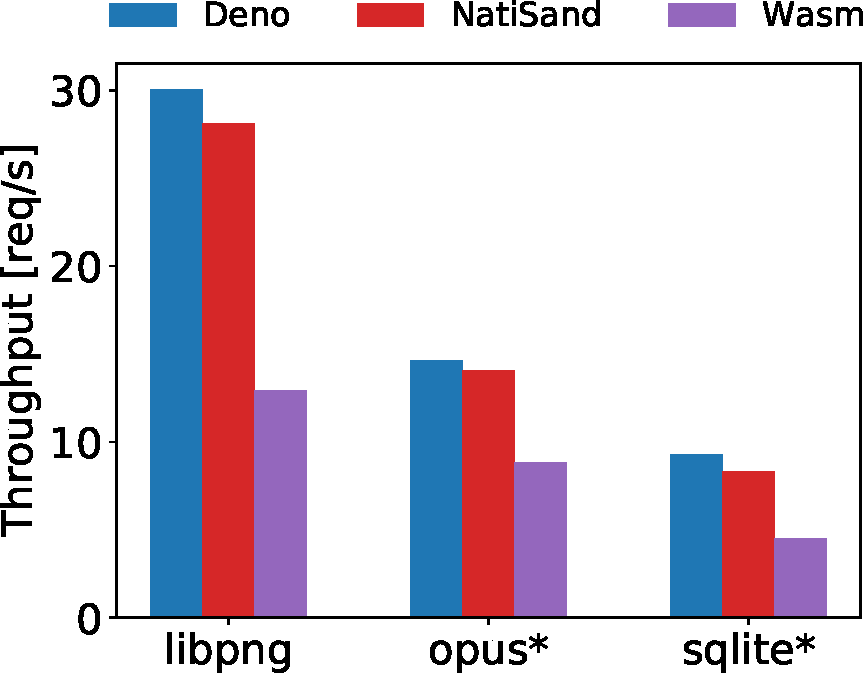
\includegraphics[width=\columnwidth]{chapters/natisand/fig/cropped-summary-ffi-throughput.pdf}
	\end{subfigure}
	\caption[Average latency and throughput of native-functions-based
		microservices]{
		Average latency and throughput for microservices that execute
		native functions (* marks the use of {\tt nativeCall})
	}
	\label{fig:native-lib-latecy-throughput}
\end{figure}

\paragraph{Usability}
%
While Wasm offers strong isolation guarantees, it also comes with drawbacks compared to \natisand. First of all it requires the developer
to use a Wasm-compatible version of the library. In our evaluation we
used a precompiled version of sqlite3, but we had to manually compile
opus and libpng using the Emscripten toolchain~\cite{emscripten} and
the WASI Sdk~\cite{wasi-sdk}, respectively. Moreover, current implementations of the WebAssembly
System Interface (WASI) can only restrict ambient rights
programmatically, and filesystem privileges work at
directory granularity. Lastly, Wasm requires the developer to
explicitly allocate, write, and read bytes from the Wasm module linear
memory.


%%% Local Variables:
%%% mode: latex
%%% TeX-master: "../main.tex"
%%% End:
